% \vspace{-20pt}

\section{主要学术成绩概述}
% \noindent\emph{\large{}主要学术成绩概述}\\[-24pt]

凝聚态体系中的\emph{激发态动力学}是决定凝聚态物质性质的关键,从时间、空间、能量、
动量、自旋等多个维度来理解乃至于调控凝聚态体系的超快动力学过程是现代凝聚态物理重
要的新兴方向之一,其中第一性原理计算软件是不可或缺的工具。申请人自2016年在中国科
大工作以来,\emph{聚焦凝聚态体系激发态动力学程序的发展与推广},取得了一系列重要的
成果,包括:
\begin{enumerate}
[
leftmargin=20pt,
label=\textnormal{[\arabic*]}
]
\kaishu{}
  
\item \emph{为第一性原理激发态动力学程序包\hnamd{}的发展做出重要贡献}。\hnamd{}是
  源于国内、具有独立知识产权的凝聚态体系激发态第一性原理计算软件,近年来在国内外
  得到了广泛的应用,申请人为\hnamd{}的发展做出了如下贡献:
  \begin{enumerate*} [label=\textnormal{(\roman*)}]
  \item 作为\emph{\hnamd{}的最早开发者,搭建了\hnamd{}的程序框架},并完成了单粒子
    图像下、实空间载流子动力学程序模块;
    
  \item 引入自旋轨道耦合,发展了\hnamd{}中的\emph{自旋动力学模块},为研究自旋轨道
    耦合诱导的自旋动力学提供了工具;
    
  \item 通过引入电声耦合矩阵元,将实空间载流子动力学扩展到动量空间,\emph{实现了
      动量空间载流子动力学模拟}。
    
  % \item 参与发展自旋分辨$GW+{}$real-time BSE
  %   方法,突破了$GW+{}$BSE方法在含时动力学上的瓶颈,使固体激发态动力学可以准确包
  %   含多体效应。
  \end{enumerate*}

  % \emph{发展和推广}第一性原理激发态动力学程序包\hnamd{}。该软件包是一个具有独
  % 立知识产权、自主可控的激发态动力学第一性原理计算软件,旨在对激发态载流子动力学
  % 进行研究,聚焦于电子空穴的复合、界面超快电荷转移、谷电子和谷激子动力学、动量空
  % 间载流子动力学等问题,在光电器件以及清洁能源材料等领域有重要的应用。申请人贡献
  % 了该程序的\emph{初版的主要代码和框架,并指导增加后续其他功能},比如\emph{率先实
  %   现了自旋分辨的$GW+{}$rtBSE方法},突破了$GW+{}$BSE 方法在含时动力学上的瓶颈,
  % 使固体激发态动力学可以准确包含激子多体效应;实现了\emph{动量空间实时载流子动力
  %   学模拟(\namdk)},需要利用单胞计算电声耦合即可,\emph{大幅降低}了计算量,为
  % 研究材料中的载流子在动量空间中的动力学行为提供了有力的工具,也为研究光致相变、
  % 光催化提供了可能的技术手段。
  
\item 利用\hnamd{}系统地研究了一系列\emph{固体材料中的激发态动力学问题}:
  \begin{enumerate*} [label=\textnormal{(\roman*)}]
    
  \item 研究了\emph{不同界面体系激发态电荷的转移}的动力学过程,阐明界面激发态电子、
    声子等准粒子相互耦合的复杂超快过程中的物理机制;

  \item 定量研究了\emph{半导体材料中的电子空穴复合}中心的形成机制,为设计高效率的
    光电器件材料做出了理论预言;
    
  % \item 研究了一系列\emph{表面吸附单分子激发态动力学},为单分子激发态动力学提供了
  %   时间、空间和能量等多个维度的物理图像。
    
  % \item 研究了三维及二维磁性材料自旋轨道耦合诱导的自旋动力学,为设计超快光控自旋
  %   器件提供了方案。
    
  \item 研究了不同材料中的极化子动力学,给出了凝聚态体系光激发极化子在时间、空间、
    能量等多个维度上的物理图像。
  \end{enumerate*}
  \emph{这些工作对\hnamd{}在不同领域中的应用起到了重要的示范作用,为\hnamd{}的推
    广做出了重要贡献。}
\end{enumerate}

申请人计划未来继续专注于凝聚态体系激发态动力学,在\hnamd{}原有基础上,进一步发展
计算方法,揭示新兴量子材料中激发态动力学的物理机制,力争解决更多凝聚态领域激发态
动力学的重要科学难题。

%%%%%%%%%%%%%%%%%%%%%%%%%%%%%%%%%%%%%%%%%%%%%%%%%%%%%%%%%%%%%%%%%%%%%%%%%%%%%%%%
% 共发表文章52篇,其中在【Frontiers of Data and Computing】、【Fundamental
% Research】和【Electronic Structure】上发表的3篇属于ESCI收录。
%%%%%%%%%%%%%%%%%%%%%%%%%%%%%%%%%%%%%%%%%%%%%%%%%%%%%%%%%%%%%%%%%%%%%%%%%%%%%%%%

申请人共发表SCI收录文章\emphNum{49}篇,% \emph
{
  近五年共发表论文\emphNum{35}篇,
  其中以(共同)通讯/(共同)第一作者发表
  \emphNum{1}篇{\itshape Nat.\ Comp.\ Sci.}、
  \emphNum{1}篇综述性文章{\itshape WIRES Comput.\ Mol.\ Sci.}、
  \emphNum{2}篇{\itshape Phys.\ Rev.\ B}、
  \emphNum{1}篇{\itshape Nano Lett.}、
  \emphNum{5}篇{\itshape J.\ Phys.\ Chem.\ Lett.},
  全部文章总引用次数\emphNum{2056}次,H因子\emphNum{26}(Google Scholar 数据)。
}

%%%%%%%%%%%%%%%%%%%%%%%%%%%%%%%%%%%%%%%%%%%%%%%%%%%%%%%%%%%%%%%%%%%%%%%%%%%%%%%%
\section{为第一性原理激发态动力学程序包\hnamd{}的发展做出重要贡献}
%%%%%%%%%%%%%%%%%%%%%%%%%%%%%%%%%%%%%%%%%%%%%%%%%%%%%%%%%%%%%%%%%%%%%%%%%%%%%%%%

\begin{center}
  \begin{InnovationBox}
    率先搭建了自主知识产权的第一性原理激发态动力学程序\hnamd{}的程序框架,并贡献
    了其中:i) 单粒子图像下载流子动力学; ii) 自旋动力学;iii)动量空间动力学等三个
    重要模块。此外还参与发展了自旋分辨激子动力学($GW{}+{}$real-time BSE)以及包含
    核量子效应的载流子动力学。与此同时,致力于\hnamd{}的推广,程序已得到越来越多
    的应用。
  \end{InnovationBox}
\end{center}

%%%%%%%%%%%%%%%%%%%%%%%%%%%%%%%%%%%%%%%%%%%%%%%%%%%%%%%%%%%%

% 第一性原理(first-principles)计算是人们理解凝聚态物质本质的重要工具,传统的第一
% 性原理计算基于玻恩--奥本海默近似,关注材料基态的电子结构,可以得到不同原子核的相
% 互作用势,从而进行基态的分子动力学计算。然而,\emph{考虑到激发态下的晶格、电子、
%   自旋动力学,目前并没有成熟的第一性原理计算方法与软件,这也是第一性原理计算发展
%   的新方向}。总得来说,激发态动力学模拟的基本思路是将不同层次的电子结构方法,例如
% 密度泛函理论、 线性响应含时密度泛函、$GW+{}$BSE等,与动力学的一些方法,例如含时薛定谔
% 方程、含时科恩-沈吕九方程、平均场动力学、轨迹面跳跃以及分子动力学等方法相结合,来
% 研究晶格、电子、自旋的动力学过程。

% 激发态弛豫的过程实际上描述的是与原子核运动耦合在一起的电子在不同本征态之间跃迁的
% 过程,由于\emph{涉及到不止一个势能面},这类问题显然是\emph{超越玻恩--奥本海默近
%   似}的。在化学动力学领域,包含非绝热效应的动力学方法有很长的发展历史,对于模型体
% 系或原子数非常少的小分子体系,可以用所谓“全量子”方法,也就是将原子核与电子都当成
% 量子粒子来处理。然而,\emph{全量子方法的计算量非常大},\emph{无法处理凝聚态材料体
%   系这种复杂体系}。因此,人们往往使用\emph{混合量子-经典}的非绝热动力学方法,把原
% 子核当成经典粒子、电子当成量子粒子来分开处理。这其中主要的思路有两类,一类是与平
% 均场动力学方法相结合,在平均场势能面上同时演化原子核与电子,基于这个思路发展的方
% 法其实就是实时的含时密度泛函方法。另一类被笼统地称作NAMD方法,这里人们将实时演化
% 的科恩--沈方程与面跳跃方法相结合,引入经典路径近似,利用分子动力学得到晶格演化的
% 实时轨迹,以此来模拟声子的激发,然后在此基础上模拟载流子的弛豫过程。这种方法最早
% 由美国南加州大学Oleg V. Prezhdo教授提出,并应用于固体体系。他与纽约州立大学水牛城
% 分校的A. Akimov教授共同发展了PYXAID程序,可以在单粒子图像下模拟电子或空穴的动力学
% 过程。\emph{在这个理论框架的基础上,申请人所在中国科学技术大学的赵瑾教授研究组发
%   展了\hnamd{}(\url{https://hefei-namd.org/})程序,并用来模拟界面电荷转移、电子
%   空穴复合等动力学过程,申请人贡献了该程序的最初版本的主要代码和框架}。

% 近年来,以过渡金属硫族化合物、黑磷等为代表的二维材料,由于其丰富的光学激发态和诸
% 多超越传统体材料的物理性质,受到了研究者的普遍关注和重视。其中,二维材料中量子限
% 域效应导致库伦作用并不能被有效屏蔽,电子空穴间的库伦作用比较强,由此产生了各种各
% 样有意思的多体效应,比如形成各种各样的激子:亮激子、暗激子、谷激子和层间激子等。
% 针对这个问题,2021年我们将单体的实时科恩--沈方程替换为两体实时BSE方程,
% 在\hnamd{}中实现了$GW{}+{}$rtBSE--NAMD方法,进一步引入了自旋轨道耦合,可以用来研
% 究光激发之后的自旋分辨激子弛豫动力学,\emph{文章发表在\textit{Sci.\ Adv.}上,申请
%   人在其中起了重要的作用}。


% 在传统的NAMD框架下研究具有周期性边界条件的固体,人们常常使用\emph{超胞
%   法}和\emph{分子动力学}来模拟固体中声子的激发。由于使用了周期性边界条件,只有超
% 胞的$\Gamma$点的声子才会被激发,而超胞$\Gamma$点的声子又是由单胞中某些满
% 足\emph{折叠条件}的声子折叠过去的。这就导致了使用该方法模拟所包含的电声散射中涉及
% 到电子动量$\mathbf{k}$和声子动量$\mathbf{q}$点\emph{受到超胞大小的限制},对于电子
% 和声子色散比较强的体系会产生较大的困难。为了解决这个问题,2023年申请人所在研究团
% 队在\hnamd{}中将电声耦合矩阵元引入含时演化哈密顿量,实现了动量空间的非绝热动力
% 学(\namdk{})方法。他们用这种方法研究了石墨烯体系的热电子弛豫过程,与实验得到了较
% 为一致的结果。\emph{文章发表在2023年的\textit{Nat.\ Comp.  Sci.}上,申请人为共同
%   通讯作者}。与此几乎同时,上海科技大学的郑帆教授与半导体所的汪林望研究员通过引入
% 声子的平带近似,也实现了一种多$\mathbf{k}$点的NAMD方法。

凝聚态物质的晶格、电子、自旋决定了物质的基本性质。当凝聚态物质处于电场、磁场、光
场、温度等外场的作用下时,其晶格、电子、自旋往往不再处于稳定的基态,而是处于一个
非平衡的“激发态”上,此时,凝聚态物质的性质往往由其激发态动力学所决定。因
此,\emph{凝聚态物质的激发态动力学是凝聚态物理的新兴重要方向},也是未来光电器件、
光伏器件、自旋器件与能源材料研发的科学基础。

第一性原理计算是人们理解凝聚态物质的重要工具,电子结构计算、基态分子动力学等方法
已经在凝聚态物理领域取得巨大的成功。然而,针对凝聚态体系激发态动力学的第一性原理
程序发展才刚刚起步。主要原因是因为凝聚态体系的激发态动力学是\emph{一个非常复杂的、
  富有挑战的科学问题}。首先,所谓非平衡激发态是一个不稳定的状态,需要引入时间尺度,
在动力学层面上对其进行描述;其次,凝聚态物质中晶格、电子、自旋之间的相互作用,例
如电声耦合、自旋轨道耦合、激子效应等都会对激发态动力学产生影响。发展针对凝聚态体
系的第一性原理计算激发态动力学方法与程序,同时给出晶格、电子、自旋在时间、空间、
能量、动量等多维度的动力学信息,是我们长期的研究目标。

针对上述目标,申请人所在课题组发展了具有独立知识产权的、针对凝聚态体系激发态动力
学的第一性原理计算程序\hnamd{},\emph{申请人是\hnamd{}最早的开发者},在\hnamd{}发
展中做出如下贡献:



% 在发展程序的同时,\emph{申请人还致力于程序的推广},2018至2023年在“凝聚态物质激发
% 态研讨会”上进行了\emphNum{5}次规模在\emphNum{100}人左右的软件培训。至今为
% 止,\hnamd{}的用户包括美国科学院院士 Shaul Mukamel、澳大利亚科学院院士 Shixue
% Dou、爱荷华州立大学的Kaiming Ho、伦敦皇家学院的 Aron Walsh、卡内基梅隆大学的 Noa
% Marom、纽约州立大学的 A. Akimov、中国科学技术大学杨金龙院士、东南大学王金兰教授、
% 华南师范大学赵纪军教授(原就职于大连理工大学)、山东大学赵明文教授等数十个研究
% 组。
% % 例如,东南大学王金兰课题组用来计算异质结电子空穴分离与复合的效率,由此设计Z型光
% % 催化材料 [\textit{ACS Catalysis} 20, 1976 (2020)];中国科学技术大学的朱彦武教授
% % 用来研究双层石墨烯热电子弛豫与声子的耦合 [\textit{Phys.  Rev. Lett.}, 126,
% % 027402 (2021)]等。
% 从 {\large{}2016} 年起,本领域使用\hnamd{}发表的文章数目逐年增加,如
% 图-\ref{fig:hnamd_pub_list}所示。\emph{截止2024年2月,基于 \hnamd{} 发表论文总数
%   已高达 \emphNum{169} 篇},其中不乏括 \textit{Phys. Rev.  Lett.},\textit{Nat.
%   Commun.},\textit{Sci.  Adv.},\textit{npj Comput.
%   Mater.},\textit{Phys. Rev.  B},\textit{PNAS},\textit{JACS},\textit{JPCL}等
% 在内的的高水平期刊。图-\ref{fig:hnamd_pub_list}列举了历年利用\hnamd{}发表的文章数,
% 以及发表文章的期刊组成,发表文章详细信息参见\textbf{附录1.1}。申请人相信,通过持
% 续的努力,比能将 \hnamd{} 发展成为源于国内、独立知识产权、自主可控、并拥有重要国
% 际影响力的第一性原理激发态动力学程序。

% \begin{enumerate}
% \item \emph{搭建了\hnamd{}的程序框架,发展了单粒子图像下的载流子动力学方法}

\subsection{搭建\hnamd{}的程序框架,发展单粒子图像下的载流子动力学方法}

\emph{作为\hnamd{}最早的开发者},申请人结合含时科恩--沈方程(Time-dependent
Kohn-Sham Equation, TDKS)方程与面跳跃方法(Surface Hopping),搭建了\hnamd{}的程
序框架,并发展了基于单粒子图像的载流子动力学方法,申请人基于此申请了\hnamd{}的软
件著作权。单粒子图像下的载流子动力学可用于研究材料界面电荷转移、电子空穴复合、热
电子弛豫等问题,\emph{是\hnamd{}被应用最多的模块}。例如,
\begin{center}
  \begin{tikzpicture}
    \node[
    align=justify, text width=0.90\textwidth,
    font=\small\kaishu,
    inner sep=0pt,
    % draw,
    CommentColor,
    ](comment){
      %%%%%%%%%%%%%%%%%%%%%%%%%%%%%%%%%%%%%%%%%%%%%%%%%%%%%%%%%%%%%%%%%%%%%%%%%%%%%%%%
      美国科学院院士、UC Irven 大学Shaul Mukamel教授利用\hnamd{}研究了施
      主-开关-受主系统中的电荷分离和系间穿越的调制问
      题[\textit{J. Phys. Chem. A}, \textbf{125}, 3088 (2021)]; \\[3pt]
      %%%%%%%%%%%%%%%%%%%%%%%%%%%%%%%%%%%%%%%%%%%%%%%%%%%%%%%%%%%%%%%%%%%%%%%%%%%%%%%%
      澳大利亚科学院院士窦世学利用\hnamd{}研究了卤氧化物界面固氮反应的光激发载流
      子的分离和复合过程[\textit{J. Phys. Chem. Lett.}, , \textbf{11}, 9304
      (2020)]; \\[3pt]
      %%%%%%%%%%%%%%%%%%%%%%%%%%%%%%%%%%%%%%%%%%%%%%%%%%%%%%%%%%%%%%%%%%%%%%%%%%%%%%%%
      中国科学技术大学杨金龙院士利用\hnamd{}研究了二维材料中光解水的材料设
      计[\textit{J. Phys. Chem. Lett.}, \textbf{13}, 1 (2022)];\\[3pt]
      %%%%%%%%%%%%%%%%%%%%%%%%%%%%%%%%%%%%%%%%%%%%%%%%%%%%%%%%%%%%%%%%%%%%%%%%%%%%%%%%
      复旦大学龚新高院士和杨吉辉教授利用\hnamd{}研究了MoS$_2$/WS$_2$异质结中的电
      荷转移与光强之间的关系[\textit{Phys. Rev. B}, \textbf{108}, 014312 (2023)];\\[3pt]
      %%%%%%%%%%%%%%%%%%%%%%%%%%%%%%%%%%%%%%%%%%%%%%%%%%%%%%%%%%%%%%%%%%%%%%%%%%%%%%%%
      东南大学王金兰课题组用来计算异质结电子空穴分离与复合的效率,由此设计Z型光催
      化材料 [\textit{ACS Catal.}, 20, 1976 (2020)]。};

    \draw[line width=2.5pt, gray]
    ($ (comment.north west) + (-12pt, 6pt) $) ++(0, -12pt)
    -- ($ (comment.north west) + (-12pt, 6pt) $)
    -- ++(6pt, 0);

    \draw[line width=2.5pt, gray]
    ($ (comment.south east) + (12pt, -6pt) $) ++(0, 12pt)
    -- ($ (comment.south east) + (12pt, -6pt) $)
    -- ++(-6pt, 0);
  \end{tikzpicture}
\end{center}
除此以外,\emph{申请人搭建的\hnamd{}程序框架也一直为后续程序发展所使用}。

% \begin{center}
%   \begin{tikzpicture}
%     \node[
%     align=justify, text width=0.90\textwidth,
%     font=\small\kaishu,
%     inner sep=0pt,
%     ](comment){
      
%       美国科学院院士、UC Irven 大学Shaul Mukamel教授利用\hnamd{}研究了施
%       主-开关-受主系统中的电荷分离和系间穿越的调制问
%       题[\textit{J. Phys. Chem. A}, \textbf{125}, 3088 (2021)];澳大利亚科学院院
%       士窦世学利用\hnamd{}研究了卤氧化物界面固氮反应的光激发载流子的分离和复合过
%       程[\textit{J. Phys. Chem. Lett.}, , \textbf{11}, 9304 (2020)]; 中国科学技
%       术大学杨金龙院士利用\hnamd{}研究了二维材料中光解水的材料设
%       计[\textit{J. Phys. Chem. Lett.}, \textbf{13}, 1 (2022)];复旦大学龚新高院
%       士和杨吉辉教授利用\hnamd{}研究了MoS$_2$/WS$_2$异质结中的电荷转移与光强之间
%       的关系[\textit{Phys. Rev. B}, \textbf{108}, 014312 (2023)];东南大学王金兰
%       课题组用来计算异质结电子空穴分离与复合的效率,由此设计Z型光催化材
%       料 [\textit{ACS Catal.}, 20, 1976 (2020)]。


%     };

%     \draw[line width=2.5pt, gray]
%     ($ (comment.north west) + (-12pt, 6pt) $) ++(0, -12pt)
%     -- ($ (comment.north west) + (-12pt, 6pt) $)
%     -- ++(6pt, 0);

%     \draw[line width=2.5pt, gray]
%     ($ (comment.south east) + (12pt, -6pt) $) ++(0, 12pt)
%     -- ($ (comment.south east) + (12pt, -6pt) $)
%     -- ++(-6pt, 0);
%   \end{tikzpicture}
% \end{center}

% \item \emph{发展了自旋轨道耦合诱导的自旋动力学方法}
\subsection{发展了自旋轨道耦合诱导的自旋动力学方法}

凝聚态体系中的自旋动力学是激发态动力学的重要组成部分,也是超快自旋器件设计的基础,
而自旋轨道耦合是影响自旋动力学的重要因素。申请人使用投影缀加波(PAW)方法,只考虑
截断半径内的贡献,计算得到自旋轨道耦合,并将其引入含时演化哈密顿量,在\hnamd{}中
实现了自旋轨道耦合诱导的自旋动力学方法,并研究了镍体系中的超快退磁过程,文章发表
在2022年的\textit{Physical Review B}上[\textit{Phys. Rev. B}, \textbf{105},
085142 (2022)],\emph{申请人是共同通讯作者,负责具体代码的实现}。自旋动力学可以由
自旋透热表象或自旋绝热表象实现,自旋透热表象使用自旋向上或向下的Kohn-Sham轨道作为
基组,自旋轨道耦合作为微扰,其大小决定了自旋发生翻转的概率,适用于自旋轨道耦合较
小的体系; 自旋绝热表象将哈密顿量对角化之后再做含时演化,使用任意方向spinor作为基
组,适用于自旋轨道耦合较大的体系。文章发表之后,自旋动力学作为\hnamd{}的新功能迅
速得到业内同行的关注与应用。不到一年时间内基于本模块已发表文章\emphNum{7}篇。

\begin{center}
  \begin{tikzpicture}
    \node[
    align=justify, text width=0.90\textwidth,
    font=\small\kaishu,
    inner sep=0pt,
    % draw,
    CommentColor,
    ](comment){
      %%%%%%%%%%%%%%%%%%%%%%%%%%%%%%%%%%%%%%%%%%%%%%%%%%%%%%%%%%%%%%%%%%%%%%%%%%%%%%%%
      德国布莱梅大学的 Thomas Frauenheim、东南大学的王金兰教授以及美国南加州大学
      的Oleg V.\ Prezhdo研究了二维铁磁半导体异质结中的超快光控反铁磁–铁磁开关
      关[\textit{Nano Lett.}, \textbf{23}, 5688(2023)];\\[3pt]
      %%%%%%%%%%%%%%%%%%%%%%%%%%%%%%%%%%%%%%%%%%%%%%%%%%%%%%%%%%%%%%%%%%%%%%%%%%%%%%%%
      捷克查尔斯大学Junjie He 等人研究了二维异质结MnPS$_3$/MnSe$_2$中的自旋弛豫过
      程[\textit{Nano Lett.}, \textbf{23}, 8348 (2023)]; \\[3pt]
      %%%%%%%%%%%%%%%%%%%%%%%%%%%%%%%%%%%%%%%%%%%%%%%%%%%%%%%%%%%%%%%%%%%%%%%%%%%%%%%%
      大连理工大学的蒋雪等人利用该功能研究了反铁磁MnPS$_3$单层中的自旋动力
      学[\textit{npj Comput. Mater.}, \textbf{9}, 107, (2023)];\\[3pt]
      %%%%%%%%%%%%%%%%%%%%%%%%%%%%%%%%%%%%%%%%%%%%%%%%%%%%%%%%%%%%%%%%%%%%%%%%%%%%%%%%
      山东大学马海波教授(原就职于南京大学)研究了ZnPc/MoS$_2$中自旋轨道耦合增强
      的电子转移和自旋翻转[\textit{J. Phys. Chem. Lett.}, \textbf{13}, 4840
      (2022)]。};

    \draw[line width=2.5pt, gray]
    ($ (comment.north west) + (-12pt, 6pt) $) ++(0, -12pt)
    -- ($ (comment.north west) + (-12pt, 6pt) $)
    -- ++(6pt, 0);

    \draw[line width=2.5pt, gray]
    ($ (comment.south east) + (12pt, -6pt) $) ++(0, 12pt)
    -- ($ (comment.south east) + (12pt, -6pt) $)
    -- ++(-6pt, 0);
  \end{tikzpicture}
\end{center}

% 1. Nanotechnology, vol. 34, no. 28, p. 285 703, Jul. 2023.
% 2. Chinese Phys. B, vol. 33, no. 1, p. 016 301, Dec. 2023.
% 3. J. Phys. Chem. Lett., vol. 13, no. 22, pp. 4840–4848, Jun. 2022.
% 4. npj Comput. Mater., vol. 9, no. 1, p. 107, Jun. 2023.
% 5. J. Phys. D. Appl. Phys., vol. 56, no. 3, p. 035 501, Jan. 2023.
% 6. Nano Lett. 2023, 23, 12, 5688–5695


% \item \emph{发展了动量空间动力学方法}
\subsection{发展了动量空间动力学方法}

在最初的\hnamd{}框架中,程序使用实空间分子动力学来模拟声子的激发以及电子--声子散
射,由于周期性边界条件的限制,只能模拟$\Gamma$点(声子动量$\mathbf{k}=0$)的声子,
想要模拟其他动量的声子及电声散射,需要使用超胞,超胞的大小决定了\textbf{k}点的密
度。这使得\emph{原有的方法无法模拟密集的\textbf{k}点之间的电声散射,也不容易直接
  得到动量空间载流子动力学的图像}。申请人通过在简谐近似下将电子态波函数用透热基组
展开,将电声耦合矩阵元直接引入哈密顿量,用以代替之前从分子动力学计算出发得到的非
绝热耦合矩阵,从而在\hnamd{}中实现了动量空间实时载流子量子动力学的模拟(方法简
称\namdk{})。与过去的非绝热分子动力学方法相比,\emph{\namdk{}方法不需要使用超胞
  进行分子动力学计算,只需要利用单胞计算电声耦合即可,大幅度降低了计算量}。另外,
这种方法除了可以模拟电子/空穴在动量空间的动力学过程,还可以得到载流子弛豫过程中声
子激发的信息,从而为光致相变以及光催化的研究提供有力的工具。文章发表
在2023年的\textit{Nature Computational Science} 上。[\textit{Nat. Comput. Sci.},
\textbf{3}, 532 (2023)],\emph{申请人是共同通讯作者,负责代码的实现}。文章发表之
后,迅速引起业内同行的关注,加州理工大学的Marco Bernardi为本文在\textit{Nature
  Computational Science}上撰写了News \& Views [\textit{Nat. Comput. Sci.},
\textbf{3}, 480 (2023)],其中提到:

\begin{figure}
  \centering
  % 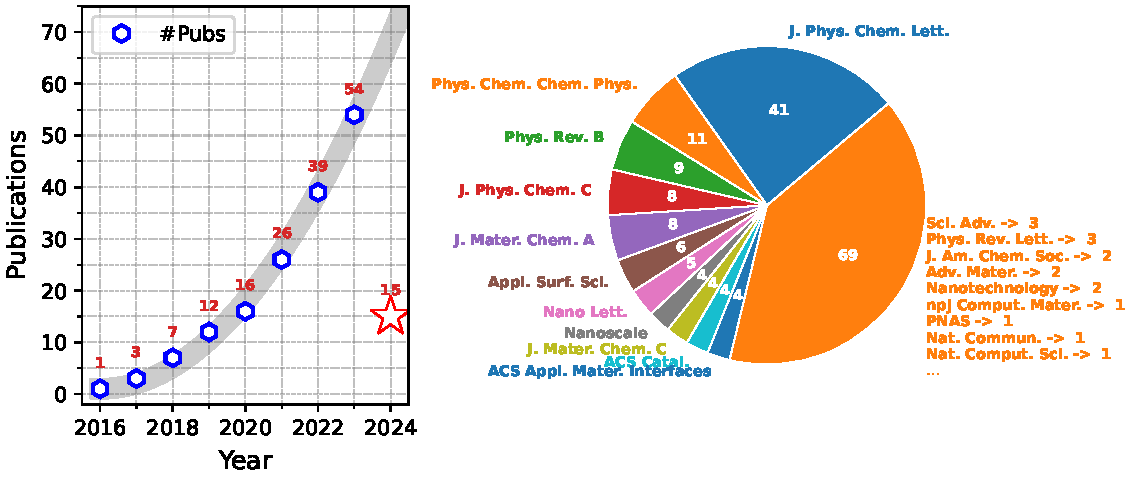
\includegraphics[width=1.0\linewidth]{figs/hefei-namd_pub_v3.pdf}
  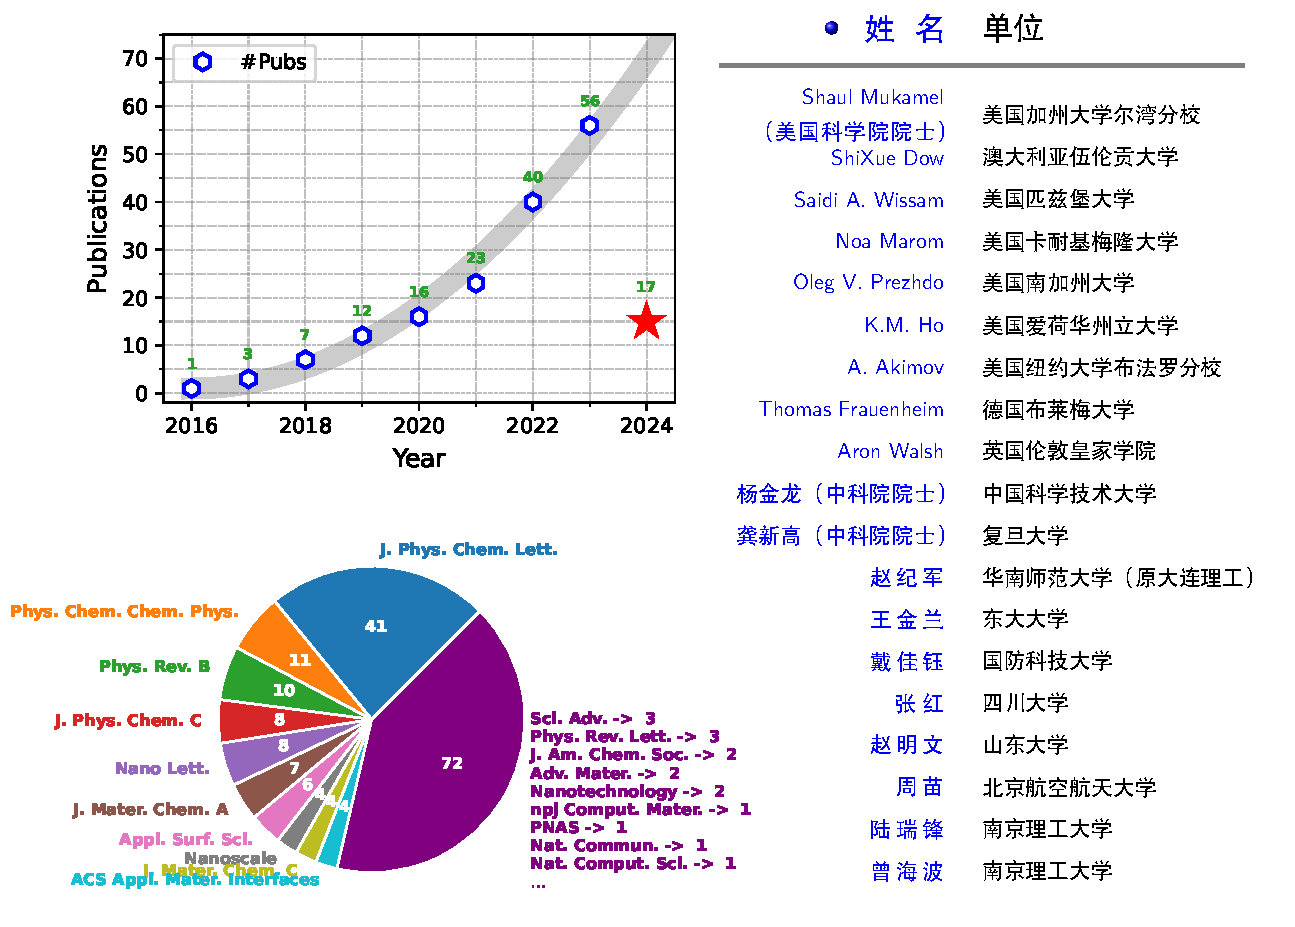
\includegraphics[width=1.0\linewidth]{figs/tikz/hefei_namd_pub_with_users.pdf}
  \caption{\label{fig:hnamd_pub_list}
    \kaishu{}%\footnotesize
    (左上)自2016年起,历年使用\hnamd{}发表的文章数,其中2024年度截止三月份已
    发表\emphNum{17}篇文章。
    (左下)使用\hnamd{}发表文章的期刊组成图,以及(右图)\hnamd{}的代表性用户。
  }
\end{figure}

\begin{center}
  \begin{tikzpicture}
    \node[
    align=justify, text width=0.90\textwidth,
    font=\small\kaishu,
    inner sep=0pt,
    CommentColor,
    ](comment){
      %%%%%%%%%%%%%%%%%%%%%%%%%%%%%%%%%%%%%%%%%%%%%%%%%%%%%%%%%%%%%%%%%%%%%%%%%%%%%%%%
      ``\ldots{}郑及其同事提出了一种动量(\textbf{k})空间方法,命名
      为\namdk{},\emph{该方法可以仅使用一个晶胞来计算电子动态,规避了昂贵的超晶
        胞计算所带来的限制}。作者演示了\namdk{}可以应用于探测热电子与声子之间任意
      动量的相互作用,这通常被认为是实空间方法无法达到的任务\ldots{}\ldots{}利用
      实时玻尔兹曼方程,人们可以提取主要的散射过程,了解主要是哪些晶格振动影响电
      子动力学,并计算受光激发的材料如何返回平衡态。\emph{郑等人做出的关键进展是,
        这些信息也可以通过非绝热时间相关的密度泛函理论获得}\ldots{}''

    };

    \draw[line width=2.5pt, gray]
    ($ (comment.north west) + (-12pt, 6pt) $) ++(0, -12pt)
    -- ($ (comment.north west) + (-12pt, 6pt) $)
    -- ++(6pt, 0);

    \draw[line width=2.5pt, gray]
    ($ (comment.south east) + (12pt, -6pt) $) ++(0, 12pt)
    -- ($ (comment.south east) + (12pt, -6pt) $)
    -- ++(-6pt, 0);
  \end{tikzpicture}
\end{center}

% \end{enumerate}

除此以外,申请人还参与发展了自旋分辨的$GW{}+{}$real-time BSE激子动力学方
法[\textit{Sci. Adv.}, \textbf{7}, eabf3759 (2021)],以及包含核量子效应
的NAMD方法[\textit{Sci. Adv.}. \textbf{8}, eabo2675 (2022)],负责指导学生实现具体
代码。\emph{在发展程序的同时,申请人还致力于程序的推广},2018至2023年在“凝聚态物
质激发态研讨会”上进行了\emphNum{5}次规模在\emphNum{100}人左右的软件培训。至今为
止,\hnamd{}的用户包括美国科学院院士 Shaul Mukamel、澳大利亚科学院院士 Shixue
Dou、爱荷华州立大学的Kaiming Ho、伦敦皇家学院的 Aron Walsh、卡内基梅隆大学的 Noa
Marom、纽约州立大学的 A. Akimov、中国科学技术大学杨金龙院士、东南大学王金兰教授、
华南师范大学赵纪军教授(原就职于大连理工大学)、国防科大戴佳钰教授、山东大学赵明
文教授等数十个研究组。截止2024年3月,基于 \hnamd{} 发表论文总数已高
达 \emphNum{175} 篇,其中不乏括 \textit{Phys.\ Rev.\ Lett.},\textit{Nat.\
  Commun.},\textit{Sci.\ Adv.},\textit{npj Comput.\ Mater.},\textit{Phys.\
  Rev.\ B},\textit{PNAS},\textit{JACS},\textit{JPCL}等在内的的高水平期
刊。\textbf{图-\ref{fig:hnamd_pub_list}}列举了历年利用\hnamd{}发表的文章数、发表
文章的期刊组成、以及\hnamd{}的代表性用户。发表文章详细信息参见\textbf{附录1}。
  

%%%%%%%%%%%%%%%%%%%%%%%%%%%%%%%%%%%%%%%%%%%%%%%%%%%%%%%%%%%%%%%%%%%%%%%%%%%%%%%%
\section{研究了不同固体材料激发态载流子动力学}
%%%%%%%%%%%%%%%%%%%%%%%%%%%%%%%%%%%%%%%%%%%%%%%%%%%%%%%%%%%%%%%%%%%%%%%%%%%%%%%%
\begin{center}
  \begin{InnovationBox}
    % 研究了不同固体材料中的激发态载流子动力学,包括:研究了不同界面体系激发态电荷
    % 的转移的动力学过程,阐明界面激发态电子、声子等准粒子相互耦合的复杂超快过程中
    % 的物理机制;定量研究了半导体材料中的电子空穴复合中心的形成机制,为设计高效率
    % 的光电器件材料做出了理论预言;
    % % 研究了三维及二维磁性材料自旋轨道耦合诱导的自旋动力学,为设计超快光控自旋器件提供了方案。
    % 研究了一系列表面吸附单分子激发态动力学,为单分子激发态动力学提供了时间、空间
    % 和能量等多个维度的物理图像。
    研究了不同固体材料中的激发态载流子动力学,为\hnamd{}的应用做出了示范,包括:研
    究了不同界面体系激发态电荷的转移的动力学过程,阐明界面激发态电子、声子等准粒
    子相互耦合的复杂超快过程中的物理机制;定量研究了半导体材料中的电子空穴复合中
    心的形成机制,为设计高效率的光电器件材料做出了理论预言;研究了不同材料中的极
    化子动力学,给出了凝聚态体系光激发极化子在时间、空间、能量等多个维度上的物理
    图像。
  \end{InnovationBox}
\end{center}

\begin{figure}
  \centering
  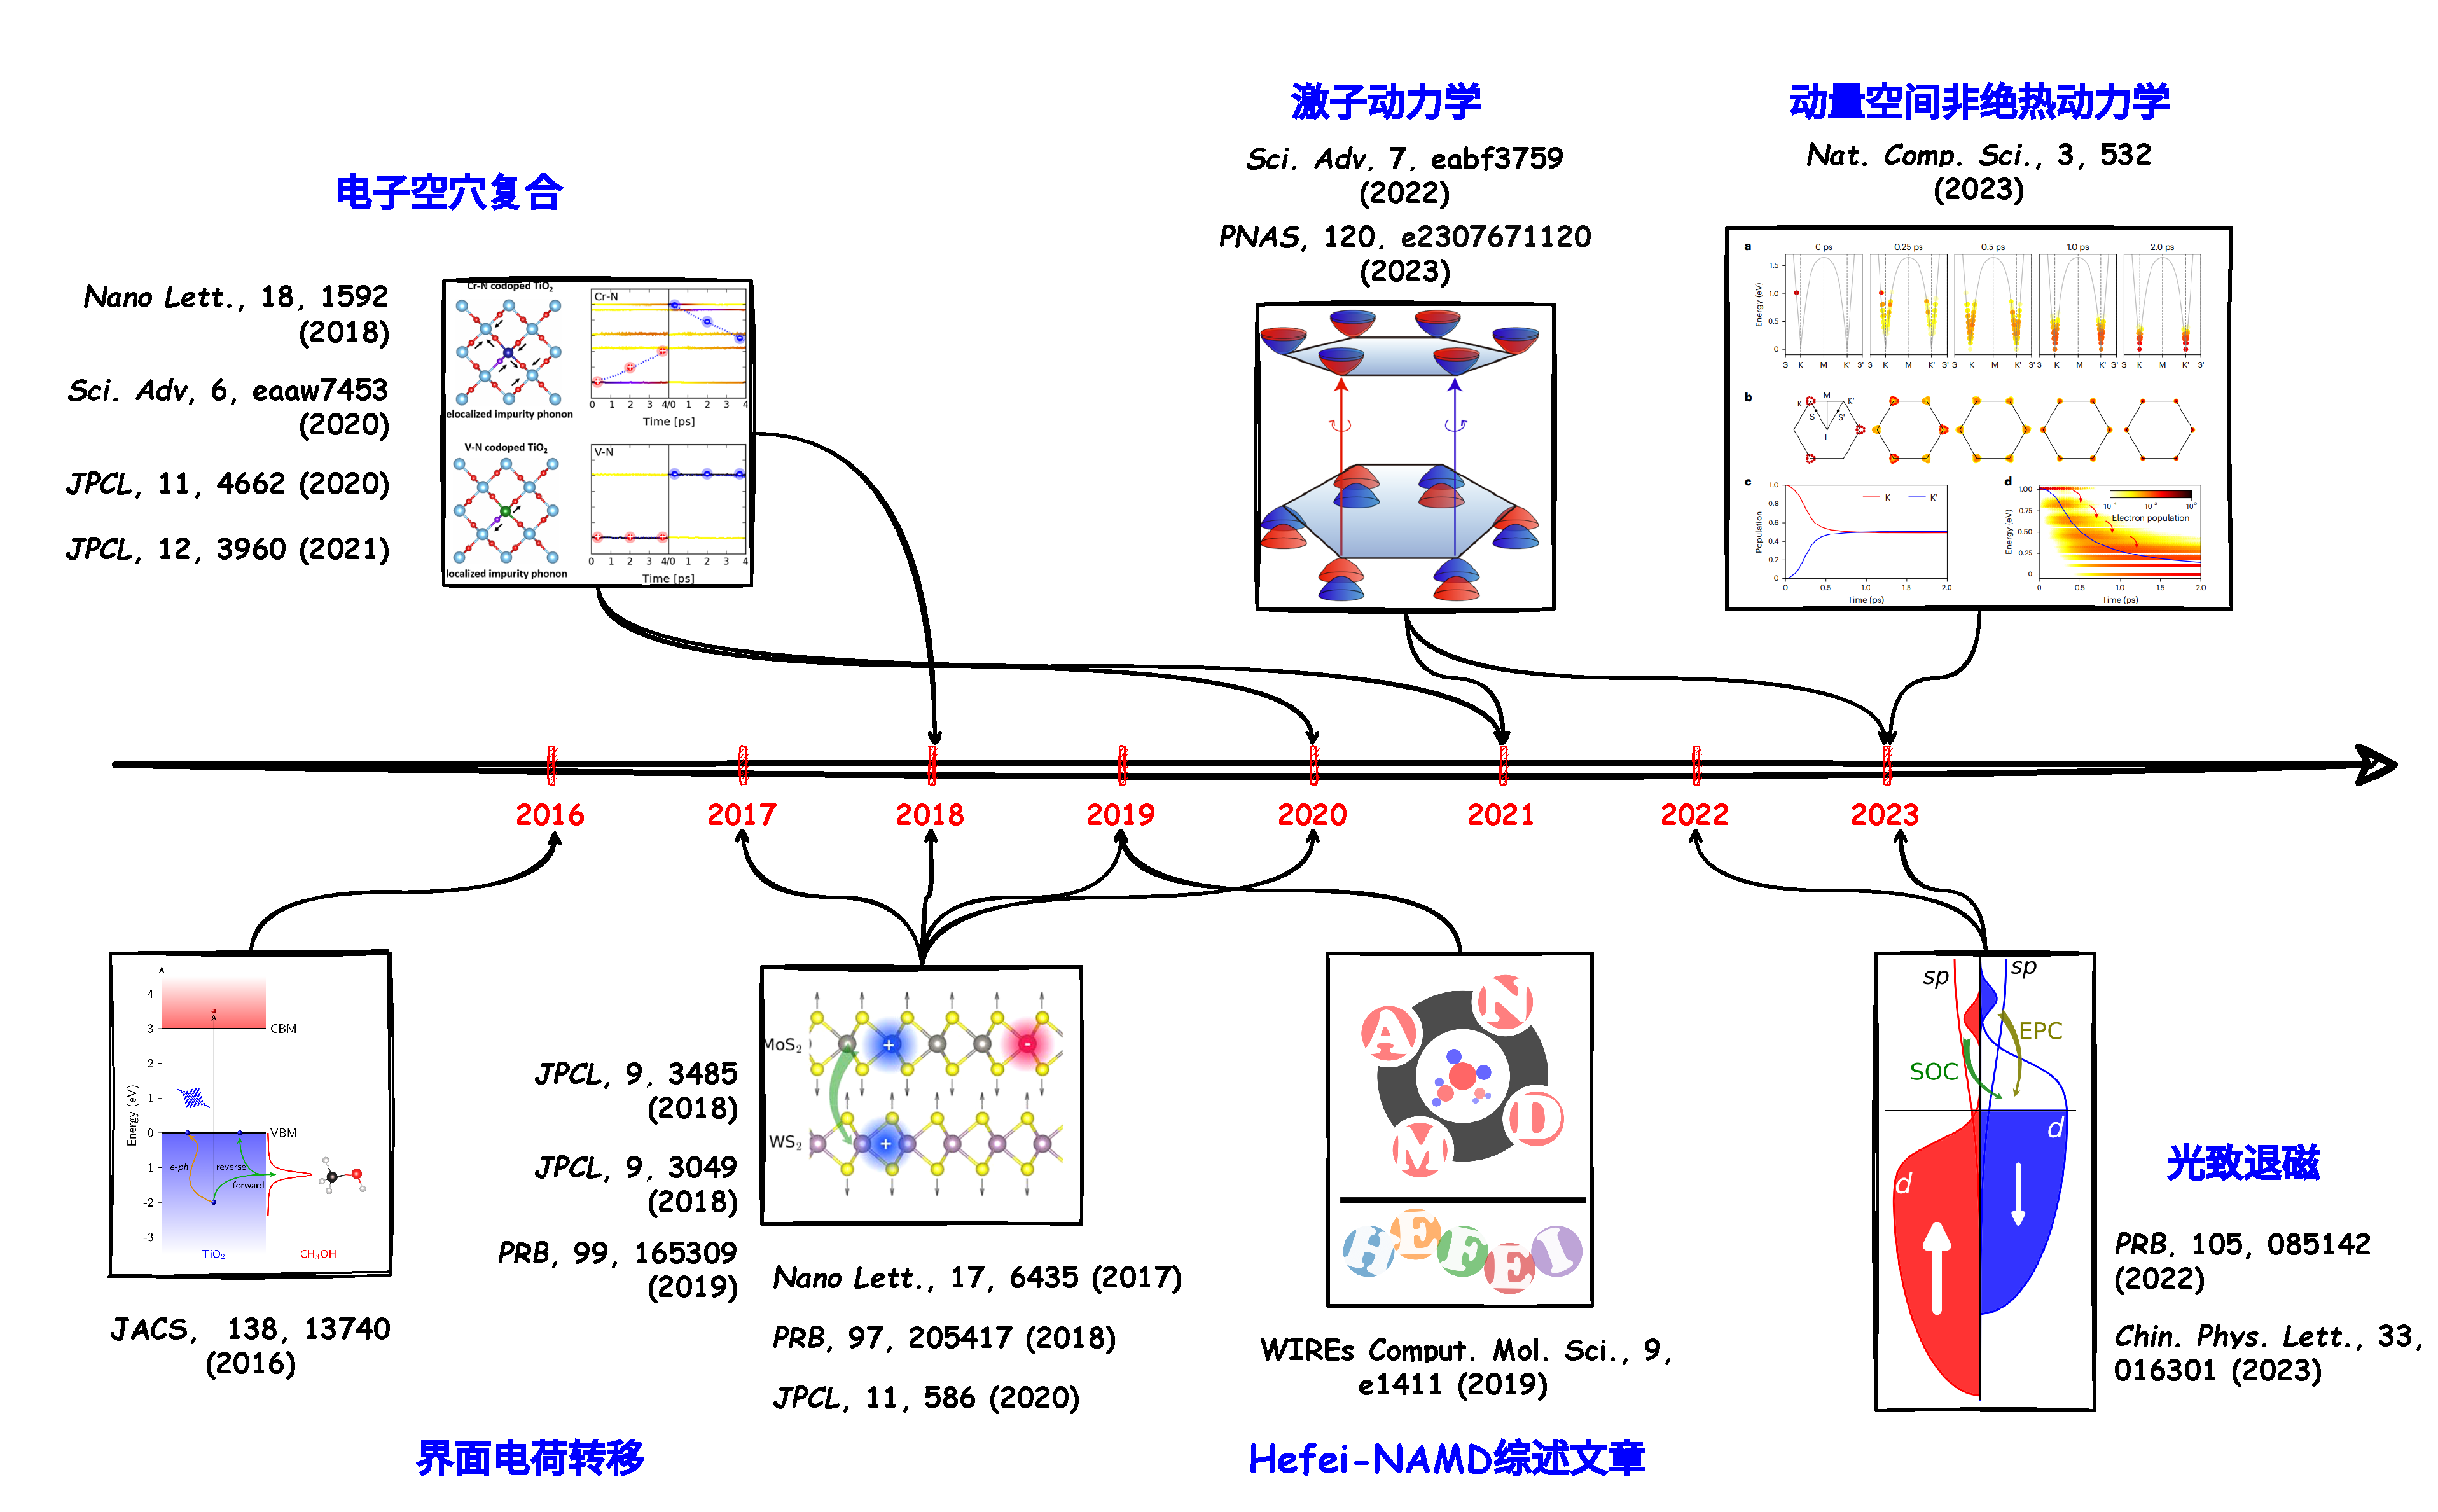
\includegraphics[width=1.\linewidth]{figs/rep_work.pdf}
  \caption{\label{fig:fig_rep_work}
    \kaishu{}%\footnotesize
    申请人历年利用Hefei-NAMD做出的一些重要工作总结。
  }
\end{figure}


固体材料中的激发态载流子动力学是影响光电及能源器件效率的关键之一。在太阳能电池、
光电器件、表面等离激元以及光催化等领域,激发态载流子的动力学行为决定了材料与器件
的效率,理解了激发态动力学行为,才有可能解决能源材料与器件领域的重要问题。申请人
分别在界面电荷转移、半导体电子空穴复合、自旋动力学等方向取得了一系列成就,成果总
结于\textbf{图-\ref{fig:fig_rep_work}}中,现就其中几个方面的工作重点展开:

%%%%%%%%%%%%%%%%%%%%%%%%%%%%%%%%%%%%%%%%%%%%%%%%%%%%%%%%%%%%%%%%%%%%%%%%%%%%%%%%
\subsection{提出范德华异质结超快界面电荷转移物理机制}
%%%%%%%%%%%%%%%%%%%%%%%%%%%%%%%%%%%%%%%%%%%%%%%%%%%%%%%%%%%%%%%%%%%%%%%%%%%%%%%%

% \begin{enumerate}[label=\textnormal{\color{EmphColor}\Roman*.}]
% \item {\color{EmphColor}\kaishu\bfseries{}
%     提出范德华异质结、金属纳米颗粒/半导体超快界面电荷转移物理机制
% }


%   Nano Lett., 17, 6435 (2017)
% https://webofscience.clarivate.cn/wos/woscc/full-record/WOS:000413057500080   

在二维材料兴起之后,范德华异质结材料由于其在光电器件领域的潜力受到了人们大量的关
注,这类界面相互作用很弱,不存在化学键,但多个实验组都证明界面存在时间尺度在数十
飞秒的超快电荷转移,这其中的物理机制人们还无法理解。我们利用 \hnamd{} 研究了过渡
金属硫族化物(TMD)界面的电荷转移过程,发现电声耦合在界面电荷转移中起到了非常重要
的作用,在 MoS$_2$/WS$_2$ 界面,光学支声子的辅助是空穴超快转移的重要原
因[\textit{Nano Lett.} \textbf{17}, 6435 (2017)](引用\emphNum{196}次,\textbf{附
  录2}),在 MoSe$_2$/WSe$_2$ 界面,由于更强的电声耦合,甚至会发生声子耦合的界面电
荷振荡[\textit{Phys.\ Rev.\ B}, \textbf{97}, 205417 (2018)]。我们还进一步提出可以
通过施加应力的方法调控界面电荷转移的时间尺度[\textit{J.\ Phys.\ Chem.\ Lett.},
\textbf{11}, 586 (2020)]。\emph{这些工作成功地揭示了声子激发以及电声耦合在界面电
  荷转移动力学中的重要作用。}

\begin{center}
  \begin{tikzpicture}
    \node[
    align=justify, text width=0.90\textwidth,
    font=\small\kaishu,
    inner sep=0pt,
    % draw,
    CommentColor,
    ](comment){
      %%%%%%%%%%%%%%%%%%%%%%%%%%%%%%%%%%%%%%%%%%%%%%%%%%%%%%%%%%%%%%%%%%%%%%%%%%%%%%%%
      我们提出的声子辅助电荷转移的机制被哥伦比亚大学 Howard Family 教授 X.Y.
      Zhu的时间分辨超快实验证实,他们直接观察到了电荷转移与声子的耦
      合[\textit{Phys.\ Rev.\ B}, 101, 201405 (2020)], 声子辅助超快电荷转移这一概
      念也被广泛接受,德国巴伐利亚科学院院士 U.
      H\"ofer 教授[\textit{Phys. Rev. B}, 102, 125417(2020), \textit{Nanoscale},
      5, 1603 (2020)],德国马普所的 Gierz 教授[\textit{Sci. Adv.}, 6, eaay0761
      (2020)], 及浙江大学的朱海明教授[\textit{J. Phys. Chem. Lett.}, 10, 150
      (2019)] 用我们提出的概念成功地解释了他们的实验结果。
      % 2019 年被 Web of
      % Science 评为诺奖热门人选的斯坦福大学Tony Heinz 教授在其发表
      % 在\textit{Nat. Nanotech.}上的综述中评价到:“最近一些工作证实了声子在电荷转
      % 移中的直接作用\ldots{}人们认为声子可以将电子从K谷散射搞$\Gamma$谷,此时层间
      % 有更强的杂化,有助于电荷转移的发生\ldots{}Zheng等人利用TDDFT方法证实了这个
      % 原理。”[\textit{Nat.\ Nanotech.}, 57, 5320 (2018)]。

    };

    \draw[line width=2.5pt, gray]
    ($ (comment.north west) + (-12pt, 6pt) $) ++(0, -12pt)
    -- ($ (comment.north west) + (-12pt, 6pt) $)
    -- ++(6pt, 0);

    \path[line width=2.5pt, gray]
    ($ (comment.south east) + (12pt, -6pt) $) ++(0, 12pt)
    -- ($ (comment.south east) + (12pt, -6pt) $)
    -- ++(-6pt, 0);
  \end{tikzpicture}
  \begin{tikzpicture}
    \node[
    align=justify, text width=0.90\textwidth,
    font=\small\kaishu,
    inner sep=0pt,
    % draw,
    CommentColor,
    ](comment){
      %%%%%%%%%%%%%%%%%%%%%%%%%%%%%%%%%%%%%%%%%%%%%%%%%%%%%%%%%%%%%%%%%%%%%%%%%%%%%%%%
      % 我们提出的声子辅助电荷转移的机制被哥伦比亚大学 Howard Family 教授 X.Y.
      % Zhu的时间分辨超快实验证实,他们直接观察到了电荷转移与声子的耦
      % 合[\textit{Phys.\ Rev.\ B}, 101, 201405 (2020)], 声子辅助超快电荷转移这一概
      % 念也被广泛接受,德国巴伐利亚科学院院士 U.
      % H\"ofer 教授[\textit{Phys. Rev. B}, 102, 125417(2020), \textit{Nanoscale},
      % 5, 1603 (2020)],德国马普所的 Gierz 教授[\textit{Sci. Adv.}, 6, eaay0761
      % (2020)], 及浙江大学的朱海明教授[\textit{J. Phys. Chem. Lett.}, 10, 150
      % (2019)] 用我们提出的概念成功地解释了他们的实验结果。
      2019 年被 Web of Science 评为诺奖热门人选的斯坦福大学Tony Heinz 教授在其发
      表在\textit{Nat. Nanotech.}上的综述中评价到:“最近一些工作证实了声子在电荷
      转移中的直接作用\ldots{}人们认为声子可以将电子从K谷散射搞$\Gamma$谷,此时层
      间有更强的杂化,有助于电荷转移的发生\ldots{}Zheng等人利用TDDFT方法证实了这
      个原理。”[\textit{Nat.\ Nanotech.}, 57, 5320 (2018)]。

    };

    \path[line width=2.5pt, gray]
    ($ (comment.north west) + (-12pt, 6pt) $) ++(0, -12pt)
    -- ($ (comment.north west) + (-12pt, 6pt) $)
    -- ++(6pt, 0);

    \draw[line width=2.5pt, gray]
    ($ (comment.south east) + (12pt, -6pt) $) ++(0, 12pt)
    -- ($ (comment.south east) + (12pt, -6pt) $)
    -- ++(-6pt, 0);
  \end{tikzpicture}
\end{center}

% \begin{justify} 
%   %%%%%%%%%%%%%%%%%%%%%%%%%%%%%%%%%%%%%%%%%%%%%%%%%%%%%%%%%%%%%%%%%%%%%%%%%%%%%%%%
%   \small\kaishu\color{CommentColor}{}
%   %%%%%%%%%%%%%%%%%%%%%%%%%%%%%%%%%%%%%%%%%%%%%%%%%%%%%%%%%%%%%%%%%%%%%%%%%%%%%%%%
%   我们提出的声子辅助电荷转移的机制被哥伦比亚大学 Howard Family 教授 X.Y.  Zhu的时
%   间分辨超快实验证实,他们直接观察到了电荷转移与声子的耦合[\textit{Phys.\ Rev.\
%     B}, \textbf{101}, 201405 (2020)], 声子辅助超快电荷转移这一概念也被广泛接受,
%   德国巴伐利亚科学院院士 U.  H\"ofer 教授[\textit{Phys. Rev. B}, \textbf{102},
%   125417 (2020), \textit{Nanoscale}, \textbf{5}, 1603 (2020)],德国马普所
%   的 Gierz 教授[\textit{Sci. Adv.}, \textbf{6}, eaay0761 (2020)], 及浙江大学的朱
%   海明教授[\textit{J. Phys. Chem. Lett.}, \textbf{10}, 150 (2019)] 用我们提出的概
%   念成功地解释了他们的实验结果。2019 年被 Web of Science 评为诺奖热门人选的斯坦福
%   大学Tony Heinz 教授在其发表在\textit{Nat. Nanotech.}上的综述中评价到:“最近一些
%   工作证实了声子在电荷转移中的直接作用\ldots{}人们认为声子可以将电子从K谷散射
%   搞$\Gamma$谷,此时层间有更强的杂化,有助于电荷转移的发生\ldots{}Zheng等人利
%   用TDDFT方法证实了这个原理。”[\textit{Nat.\ Nanotech.}, \textbf{57}, 5320
%   (2018)]。
% \end{justify}

  
% \item {\color{EmphColor}\kaishu\bfseries{}
%     发现电子空穴复合中心的产生与半导体硬度的关系,提出调控载流子寿命的理论方案
%   }

\subsection{半导体中电子空穴复合动力学}

半导体材料常有的缺陷和杂质会产生电子空穴复合中心,降低器件的效率,如何通过材料设
计尽量减少半导体材料的电子空穴复合中心是这个领域的重要问题。我们研究了一系列半导
体材料中的电子空穴复合动力学,在 TiO$_2$ 为代表的氧化物半导体中,我们发现能量位于
能隙中间的深杂质能级会成为电子空穴复合中心,这与人们熟悉的 Shockley-Reed-Hall
(SRH) 模型给出的结论一致[\textit{Nano Lett.}, \textbf{18}, 1592 (2018),\emph{共
  同一作}]。然而,在有机钙钛矿太阳能电池(MAPbI$_3$)的工作中,我们却发现无论是深
能级缺陷还是浅能级缺陷,都没有形成明显的电子空穴复合中心,分析表明主要原因是由于
这种材料硬度很低,因此导带底、价带顶与缺陷能级都只与低频声子耦合,从而使得无论缺
陷是深能级还是浅能级,电子空穴复合都很慢,不会有复合中心的形成。因此,我们提出硬
度较低的半导体材料不易形成电子空穴复合中心,这类材料可能在清洁能源及光电器件方面
有重要的应用 [\textit{Sci. Adv.}, \textbf{6,} eaaw7453, (2020),第二作者]。由于电
子空穴复合主要由电声耦合所影响,我们进一步提出了通过元素掺杂或施加应力调控电子空
穴复合的理论方案。首先,通过N、As、Sb、Bi四种元素对黑磷体系的掺杂,我们发现所有的
掺杂都会缩短载流子的寿命,这是由于元素掺杂引入了一些杂质声子,缩短了激发态电子空
穴的退相干时间。我们同时发现了,掺杂的元素质量越大,载流子的寿命越长的规律。同样,
对于黑磷材料,当我们施加拉伸应力时,可以增强垂直方向声学支的激发,有效减小载流子
寿命。这两项工作为调控半导体材料中的载流子寿命提供了理论依据,文章发表
在\textit{J. Phys. Chem. Lett.}上, \emph{申请人为共同通讯[\textit{JPCL},
  \textbf{11}, 4662 (2020)]与唯一通讯作者[\textit{JPCL}, \textbf{12}, 3960
  (2021)]}。

% \begin{justify}
%   %%%%%%%%%%%%%%%%%%%%%%%%%%%%%%%%%%%%%%%%%%%%%%%%%%%%%%%%%%%%%%%%%%%%%%%%%%%%%%%%
%   \small\kaishu\color{CommentColor}{}
%   %%%%%%%%%%%%%%%%%%%%%%%%%%%%%%%%%%%%%%%%%%%%%%%%%%%%%%%%%%%%%%%%%%%%%%%%%%%%%%%%
%   这一系列文章发表后引起了业内同行的关注,苏黎世理工大学的 KovalenKo 教授用我们提
%   出的概念解释了他们的 NMR 和 NQR 实验[\textit{J. Am. Chem. Soc.}, \textbf{142},
%   19413 (2020)]。北京师范大学的方维海院士在他们的文章中用详细介绍了我们在电子空穴
%   复合方面的工作[\textit{J. Mater. Chem. A}, \textbf{8}, 25235 (2020)]: “赵与合作
%   者研究了不同材料中的电子空穴复合动力学,包括钙钛矿、金红石二氧化钛、黑磷等,为
%   设计高效光伏和光催化材料提供了重要的理论依据\ldots{}”
% \end{justify}

\begin{center}
  \begin{tikzpicture}
    \node[
    align=justify, text width=0.90\textwidth,
    font=\small\kaishu,
    inner sep=0pt,
    CommentColor,
    ](comment){
      %%%%%%%%%%%%%%%%%%%%%%%%%%%%%%%%%%%%%%%%%%%%%%%%%%%%%%%%%%%%%%%%%%%%%%%%%%%%%%%%
      这一系列文章发表后引起了业内同行的关注,苏黎世理工大学的 KovalenKo 教授用我
      们提出的概念解释了他们的 NMR 和 NQR 实验[\textit{J. Am. Chem. Soc.},
      \textbf{142}, 19413 (2020)]。\\[3pt]
      %%%%%%%%%%%%%%%%%%%%%%%%%%%%%%%%%%%%%%%%%%%%%%%%%%%%%%%%%%%%%%%%%%%%%%%%%%%%%%%%
      北京师范大学的方维海院士在他们的文章中用详细介绍了我们在电子空穴复合方面的
      工作[\textit{J. Mater. Chem. A}, \textbf{8}, 25235 (2020)]: “赵与合作者研究
      了不同材料中的电子空穴复合动力学,包括钙钛矿、金红石二氧化钛、黑磷等,为设
      计高效光伏和光催化材料提供了重要的理论依据\ldots{}”

    };

    \draw[line width=2.5pt, gray]
    ($ (comment.north west) + (-12pt, 6pt) $) ++(0, -12pt)
    -- ($ (comment.north west) + (-12pt, 6pt) $)
    -- ++(6pt, 0);

    \draw[line width=2.5pt, gray]
    ($ (comment.south east) + (12pt, -6pt) $) ++(0, 12pt)
    -- ($ (comment.south east) + (12pt, -6pt) $)
    -- ++(-6pt, 0);
  \end{tikzpicture}
\end{center}


% \subsection{表面吸附单分子激发态动力学}

% 表面分子对激发态电子空穴的捕获过程是分子光电器件的关键过程,我们利用 \hnamd{} 成
% 功地给出了表面单分子激发态动力学在时间、空间、能量等多个维度上的物理图像。
% 在 CH$_3$OH/TiO$_2$ 体系中,我们发现只有解离的 CH$_3$O 才有较强的捕获激发态空穴的
% 能力,捕获空穴的时间尺度约为 150 飞秒,空穴被CH$_3$O 捕获之后,其中一部分会在 10
% 飞秒之后重新回到 TiO$_2$,发生反向空穴转移,而分子的振动会加快 TiO$_2$ 内部热空穴
% 向价带顶的弛豫。在这个动力学过程中,分子-固体的能级匹配、声子的激发及电声耦合的大
% 小是决定分子捕获空穴20的关键因素。[\textit{J. Am. Chem. Soc.}, \textbf{138},
% 13740 (2016)] 而 TiO$_2$ 表面 CO$_2$ 分子的弯曲和非对称拉伸两种振动模式如果能够被
% 有效激发,CO$_2$ 的 LUMO 轨道则会被降低至导带底之下,并保持 150 飞秒左右的时间,
% 此时 CO$_2$ 可以在 80 飞秒之内有效捕获导带上的电子,并在之后的 30--40 飞秒 发生解
% 离形成 CO 分子。这项工作揭示了CO$_2$ 振动模式激发在光还原过程中的关键性作用,并从
% 第一性原理计算的角度对TiO$_2$ 表面 CO$_2$ 分子的光致还原的激发态动力学给出了清晰
% 的描述。[\textit{J. Am. Chem.  Soc.}, \textbf{142}, 3214, (2020)]。
  
% \begin{justify}
%   %%%%%%%%%%%%%%%%%%%%%%%%%%%%%%%%%%%%%%%%%%%%%%%%%%%%%%%%%%%%%%%%%%%%%%%%%%%%%%%%
%   \small\kaishu\color{CommentColor}{}
%   %%%%%%%%%%%%%%%%%%%%%%%%%%%%%%%%%%%%%%%%%%%%%%%%%%%%%%%%%%%%%%%%%%%%%%%%%%%%%%%%
%   针对CH$_{3}$OH/TiO$_{2}$的工作,中国科学技术大学的张群教授与罗毅教授针对这项工
%   作专门设计了时间分辨的超快光谱学实验,来研究CH$_{3}$OH/C$_{3}$N$_{4}$界面的空穴
%   捕获动力学[\textit{Angew. Chem. Int. Ed.}, \textbf{57}, 5320, (2018)]。他们在文
%   章引言部分用一整段来描述实验动机:“最近,Chu等人提出了CH$_{3}$OH/TiO$_{2}$界面
%   电荷转移的物理图像…考虑到半导体界面空穴转移动力学的独特性质,用实验来验证理论的
%   预测是非常关键的。”他们的实验验证了我们文中的主要结论: i)只有 CH$_{3}$O 可以捕
%   获空穴;ii)存在反向空穴转移的过程(附件 4.8)。杨学明院士的双光子光电子能谱实验,
%   谭世京、王兵教授的STM 实验也都初步证实了CH$_3$O捕获空穴的事
%   实[\textit{J. Phys. Chem. C}, \textbf{122}, 26512, (2018);
%   \textit{J. Phys. Chem. C}, \textbf{122}, 28805, (2018)],杨学明院士在 2019 年发
%   表在\textit{Advanced Materials} 上的综述中专门论述了本工
%   作 [\textit{Adv. Mater.}, \textbf{31}, 19011997 (2019)]。Catalan Institute of
%   Nanoscience and Nanotechnology 的 A. Migani 教授用其他的计算方法证实了我们的结
%   果 [\textit{J. Am. Chem. Soc.}, \textbf{138}, 16165 (2016)],哈佛大学
%   的 E. Kaxiras 教授与物理所孟胜研究员则在其他体系中观察到了类似的现
%   象[\textit{Nano Lett.}, \textbf{18}, 6057 (2018)]。
% \end{justify}

\subsection{光激发极化子动力学}

当材料的电声耦合足够强时,激发态载流子会与声子耦合形成极化子,以新的准粒子形式发
生弛豫。通过\hnamd{},我们发现在金红石
TiO$_2$体系中,光激发电子会在几十飞秒之内与晶格发生耦合,形成局域的小极化子,小极
化子在晶格不同位点之间的跳跃与其寿命密切相关,当温度在室温以下时,小极化子展现出
空间局域的特点,此时其寿命在纳秒量级,温度升高到\SI{700}{\kelvin}左右时,小极化子
开始在不同位点频繁跳跃,此时其寿命只有皮秒量级。我们的研究发现,在强电声耦合体系,
激发态载流子往往以极化子形式存在,因此极化子的动力学对于载流子的寿命起到决定性作
用。本工作给出了氧化物体系光激发小极化子的动力学物理图像,文章发表在\textit{J.\
  Phys.\ Chem.\ Lett.}上,\emph{申请人为通讯作者}[\textit{J. Phys. Chem. Lett.},
\textbf{12}, 2191 (2021)]。

% \begin{justify}
%   %%%%%%%%%%%%%%%%%%%%%%%%%%%%%%%%%%%%%%%%%%%%%%%%%%%%%%%%%%%%%%%%%%%%%%%%%%%%%%%%
%   \kaishu\color{CommentColor}
%   %%%%%%%%%%%%%%%%%%%%%%%%%%%%%%%%%%%%%%%%%%%%%%%%%%%%%%%%%%%%%%%%%%%%%%%%%%%%%%%%
%   加拿大蒙特利尔大学的Jeffrey Roshan De Lile教授在\textit{Adv. Theory Simul.},
%   \textbf{5}, 2100244 (2021)上大篇幅介绍了我们的工作:``最近,张等人采
%   用AIMD${}+{}$U($U=\SI{4.5}{\eV}$)研究了金红石二氧化钛中额外电子
%   在100、300和\SI{700}{K}温度下的捕获过程。他们的结果表明极化子的形成时间与温度关
%   系不大\ldots\ldots{}根据张等人的结果,电荷载流子寿命的减少归因于由于在高温下增
%   加了跳跃迁移率和离域,增加了价带最大值(VBM)和极化子之间的轨道重叠。因此,加
%   强VBM和极化子之间的非绝热耦合加速了电子-空穴复合。因此,由于抑制了电子-空穴复合,
%   太阳能电池中的温度调节可以显著提高性能\ldots''
% \end{justify}

\begin{center}
  \begin{tikzpicture}
    \node[
    align=justify, text width=0.90\textwidth,
    font=\small\kaishu,
    inner sep=0pt,
    CommentColor,
    ](comment){
      %%%%%%%%%%%%%%%%%%%%%%%%%%%%%%%%%%%%%%%%%%%%%%%%%%%%%%%%%%%%%%%%%%%%%%%%%%%%%%%%
      厦门大学田中群院士在综述[\textit{Nat. Rev. Methods Primers.}, \textbf{3},
      12 (2023)]中引用我们的文献:``目前已经产生了几种理论方法可以用来研究强关联
      体系中极化子扩散、声子激发和电子空穴复合的特性。''; 

    };

    \draw[line width=2.5pt, gray]
    ($ (comment.north west) + (-12pt, 6pt) $) ++(0, -12pt)
    -- ($ (comment.north west) + (-12pt, 6pt) $)
    -- ++(6pt, 0);

    \path[line width=2.5pt]
    ($ (comment.south east) + (12pt, -6pt) $) ++(0, 12pt)
    -- ($ (comment.south east) + (12pt, -6pt) $)
    -- ++(-6pt, 0);
  \end{tikzpicture}
  \begin{tikzpicture}
    \node[
    align=justify, text width=0.90\textwidth,
    font=\small\kaishu,
    inner sep=0pt,
    CommentColor,
    ](comment){
      %%%%%%%%%%%%%%%%%%%%%%%%%%%%%%%%%%%%%%%%%%%%%%%%%%%%%%%%%%%%%%%%%%%%%%%%%%%%%%%%
      西北工业大学王洪强教
      授(国家“万人计划”科技创新领军人才)在文中[\textit{Chemical Engineering
        Journal}, \textbf{461}, 141872 (2023)]大篇幅介绍引用我们的文章:``
      \ldots{}TiO$_2$层的小极化子,可以很容易通过光激发产生,决定了金属氧化物半导
      体的载流子输运,该极化子主要局域在Ti原子上并很难跃迁,导致较低的TiO$_2$ 载
      流子移动率。'';

    };

    \path[line width=2.5pt, gray]
    ($ (comment.north west) + (-12pt, 6pt) $) ++(0, -12pt)
    -- ($ (comment.north west) + (-12pt, 6pt) $)
    -- ++(6pt, 0);

    \path[line width=2.5pt]
    ($ (comment.south east) + (12pt, -6pt) $) ++(0, 12pt)
    -- ($ (comment.south east) + (12pt, -6pt) $)
    -- ++(-6pt, 0);
  \end{tikzpicture}
  \begin{tikzpicture}
    \node[
    align=justify, text width=0.90\textwidth,
    font=\small\kaishu,
    inner sep=0pt,
    CommentColor,
    ](comment){
      北京航天航空大学刘利民教授(国家杰青)在文
      中(\textit{J. Phys. Chem. Lett.}, \textbf{13}, 857 (2022))引用我们的文献指
      出:``TiO$_2$体系在不同温度下光激发极化子的动力学已经被研究,研究表明极化子
      在不同Ti原子之间的迁移很大程度上跟电子空穴复合被抑制有关。''
    };

    \path[line width=2.5pt, white]
    ($ (comment.north west) + (-12pt, 6pt) $) ++(0, -12pt)
    -- ($ (comment.north west) + (-12pt, 6pt) $)
    -- ++(6pt, 0);

    \draw[line width=2.5pt, gray]
    ($ (comment.south east) + (12pt, -6pt) $) ++(0, 12pt)
    -- ($ (comment.south east) + (12pt, -6pt) $)
    -- ++(-6pt, 0);
  \end{tikzpicture}
\end{center}

此外,申请人与哥伦比亚大学朱晓阳教授合作通过第一性原理计算与双光子-光电子能谱探讨
了由镜像电子引起的电荷再分配,以及瞬态铁电有序化的产生,展示了二维半金
属MoTe$_2$在铁电相和顺电相下表面镜像态电子的动力学,以及瞬态铁电有序化的产生。研
究发现MoTe$_2$中的非简谐层间切向声子对镜像电子有着明显的响应,从而产生面内切向运
动,导致远弱于镜像态红移的面外极化。同时,该声子的激发伴随着显著的电荷再分配,从
而在材料表面产生均匀的面外电偶极矩,即铁电极化,进而屏蔽镜像电子,导致其能量红移。
理论计算的结果在双光子-光电子能谱实验上得到了证实。\emph{该研究首次证明瞬态电荷可
  以诱导均匀二维铁电有序化},对铁电极化子的形成提供了实验和理论支持,并且为瞬态调
控物质铁电相提供了一种新的途径。相关论文发表在\textit{Nano Lett.}, \textbf{21},
9903 (2021)上,\emph{申请人为共同第一作者}。


2019年,申请人团队受邀为\hnamd{}的应用在\textit{Wiley Interdiscip. Rev.:
  Comput. Mol. Sci.}上撰写综述文章[\textit{Wiley Interdiscip. Rev.:
  Comput. Mol. Sci.}, \textbf{9}, e1411 (2019)],\emph{申请人为第一作者},本论文
已被引用\emphNum{185}次,参见\textbf{附录3}。

%%%%%%%%%%%%%%%%%%%%%%%%%%%%%%%%%%%%%%%%%%%%%%%%%%%%%%%%%%%%%%%%%%%%%%%%%%%%%%%%
% \end{enumerate}
